% Setup
\graphicspath{./figures}

\chapter{Systems Survey and Analysis of State-of-the-Art}
\label{chap:survey}

% Introduction
% - What will this chapter contain and what resaarch question it tries to answer
% - Survey -> Identify existing SM Systems
% - Survey -> Deep dive into the individual systems
% - Result: Qualitative analysis on existing systems
Following a general introduction to concepts relevant to this thesis in \cref{chap:background}, in this chapter, we present a literature and systems survey on the state-of-the-art \gls{sm} systems. The goal of this chapter is to provide an answer to \ref{rq-1}, \textit{How do existing \gls{sm} implementations compare?}. To identify the existing systems and objectively compare these systems, we first have to conduct a systematic survey. By using a systematic process, the results as presented in this chapter can be reproduced. The survey is conducted in two phases. The goal of the first phase is to identify existing systems in the \gls{sm} landscape. After this, we survey the literature on these individual systems. The data obtained through this survey is then synthesized and used to create a framework which compares the properties and characteristics of these state-of-the-art \gls{sm} systems. Finally, we conclude this chapter by providing an extensive analysis on the obtained qualitative results and produce an answer to the research question

% Rest of the chapter is structured as follows
% - The need for these surveys (related work)
% - Methodology used for both surveys
% - Results of 
The remainder of this chapter is structured as follows. First, in \cref{sec:survey:related-work} we discuss the related work and identify the need for a systematic systems survey. Next, in \cref{sec:survey:goals} we define the goals which we aim to achieve with the survey. After this, in \cref{sec:survey:methodology} we present and explain the methodology used to conduct this survey. Furthermore, in \cref{sec:survey:results} we present the obtained results and introduce a framework of state-of-the-art \gls{sm} systems in which they are compared based on their properties and characteristics. Concluding, \cref{sec:survey:analysis} in we provide a detailed analysis on the obtained qualitative results and establish an answer to research question \ref{rq-1}.



\section{Related Work}
\label{sec:survey:related-work}

% Discuss identified related work
% - Service Mesh survey
% - Our previously conducted survey on the k8s ecosystem
Prior to conducting a survey on the field, we examined relevant and related work on the topic. We have identified secondary literature in which authors have conducted a literature review on the state-of-the-art on \gls{sm} technology \cite{service-mesh-survey}. This review that was conducted in 2019 noted the fact that there was not a lot of formal literature on the topic and stated that their work was the first work to formally synthesize the data in the field. Previous efforts by us to systematically synthesize the data concerning the formal literature on the \gls{k8s} ecosystem found similar results. \todo{Survey: Cite prev work?} In our previous work, we presented a topical framework on research conducted in the Kubernetes ecosystem and found that most of the formal literature was related to the resource management aspects of the ecosystem. With most of the research dedicated to scheduling and scaling algorithms, several of the layers as presented in the topical framework \todo{add ref to frameowkr} had relatively little attention. One of the identified technologies that was related to the Kubernetes ecosystem, in the form of \glspl{sm}, had very little formal work conducted on it, which ultimately led to the motivation behind the research conducted in this thesis.

% Reason the need for such a survey
% - Previous attempt gave general introduction
% - Not a sytems survey
% - Comparison of only a few (Istio, Linkerd, App Mesh, Synapse) sm implementations
% - Landscape changed, new technolgies, definition might change?
Although there has been a previous effort to survey the field \cite{service-mesh-survey}, we identified several shortcomings for our goals. First, the survey conducted by Li et al. provide a generic introduction to the concept of a service mesh, its features, and the challenges and opportunities in the field. Our goal is to provide a comparison of \gls{sm} implementations through their characteristics and properties. The work conducted by Li et al. do provide some form of comparison, but do so with a focus on generic and subjective characteristics such as the maturity of the product, whether it is open-source and actively worked on and what the major advantage and disadvantage is of each platform. This provides a sharp contrast in the type of comparison that we try to conduct, which heavily emphasizes on characteristics typically associated with  \gls{sm} technologies detailing the control and data plane characteristics of such a system. Furthermore, the survey was conducted in 2019, however the landscape of \gls{sm} technologies has changed drastically since then. New \gls{sm} systems have emerged, while existing systems have evolved. Where Li et al. \cite{service-mesh-survey} have identified four different systems back in 2009, the \gls{cncf} landscape \cite{cncf-landscape}\footnote{\url{https://landscape.cncf.io/card-mode?category=service-mesh&grouping=category}} contains many more systems as is depicted in \cref{fig:cncf-landscape-sm}. This landscape only presents officially accepted \gls{cncf} projects and might not cover all the systems which are out there. Finally, recent industry based efforts altered some ideas and principles of \gls{sm} systems, changing the traditional proxy-based approaches to include  \gls{ebpf}\footnote{\url{https://ebpf.io/}} based solutions, drastically changing the data plane by including revolutionary Linux kernel technologies \cite{istio-merbridge, cilium-ebpf-mesh}.


\begin{figure*}[t]
    \centering
    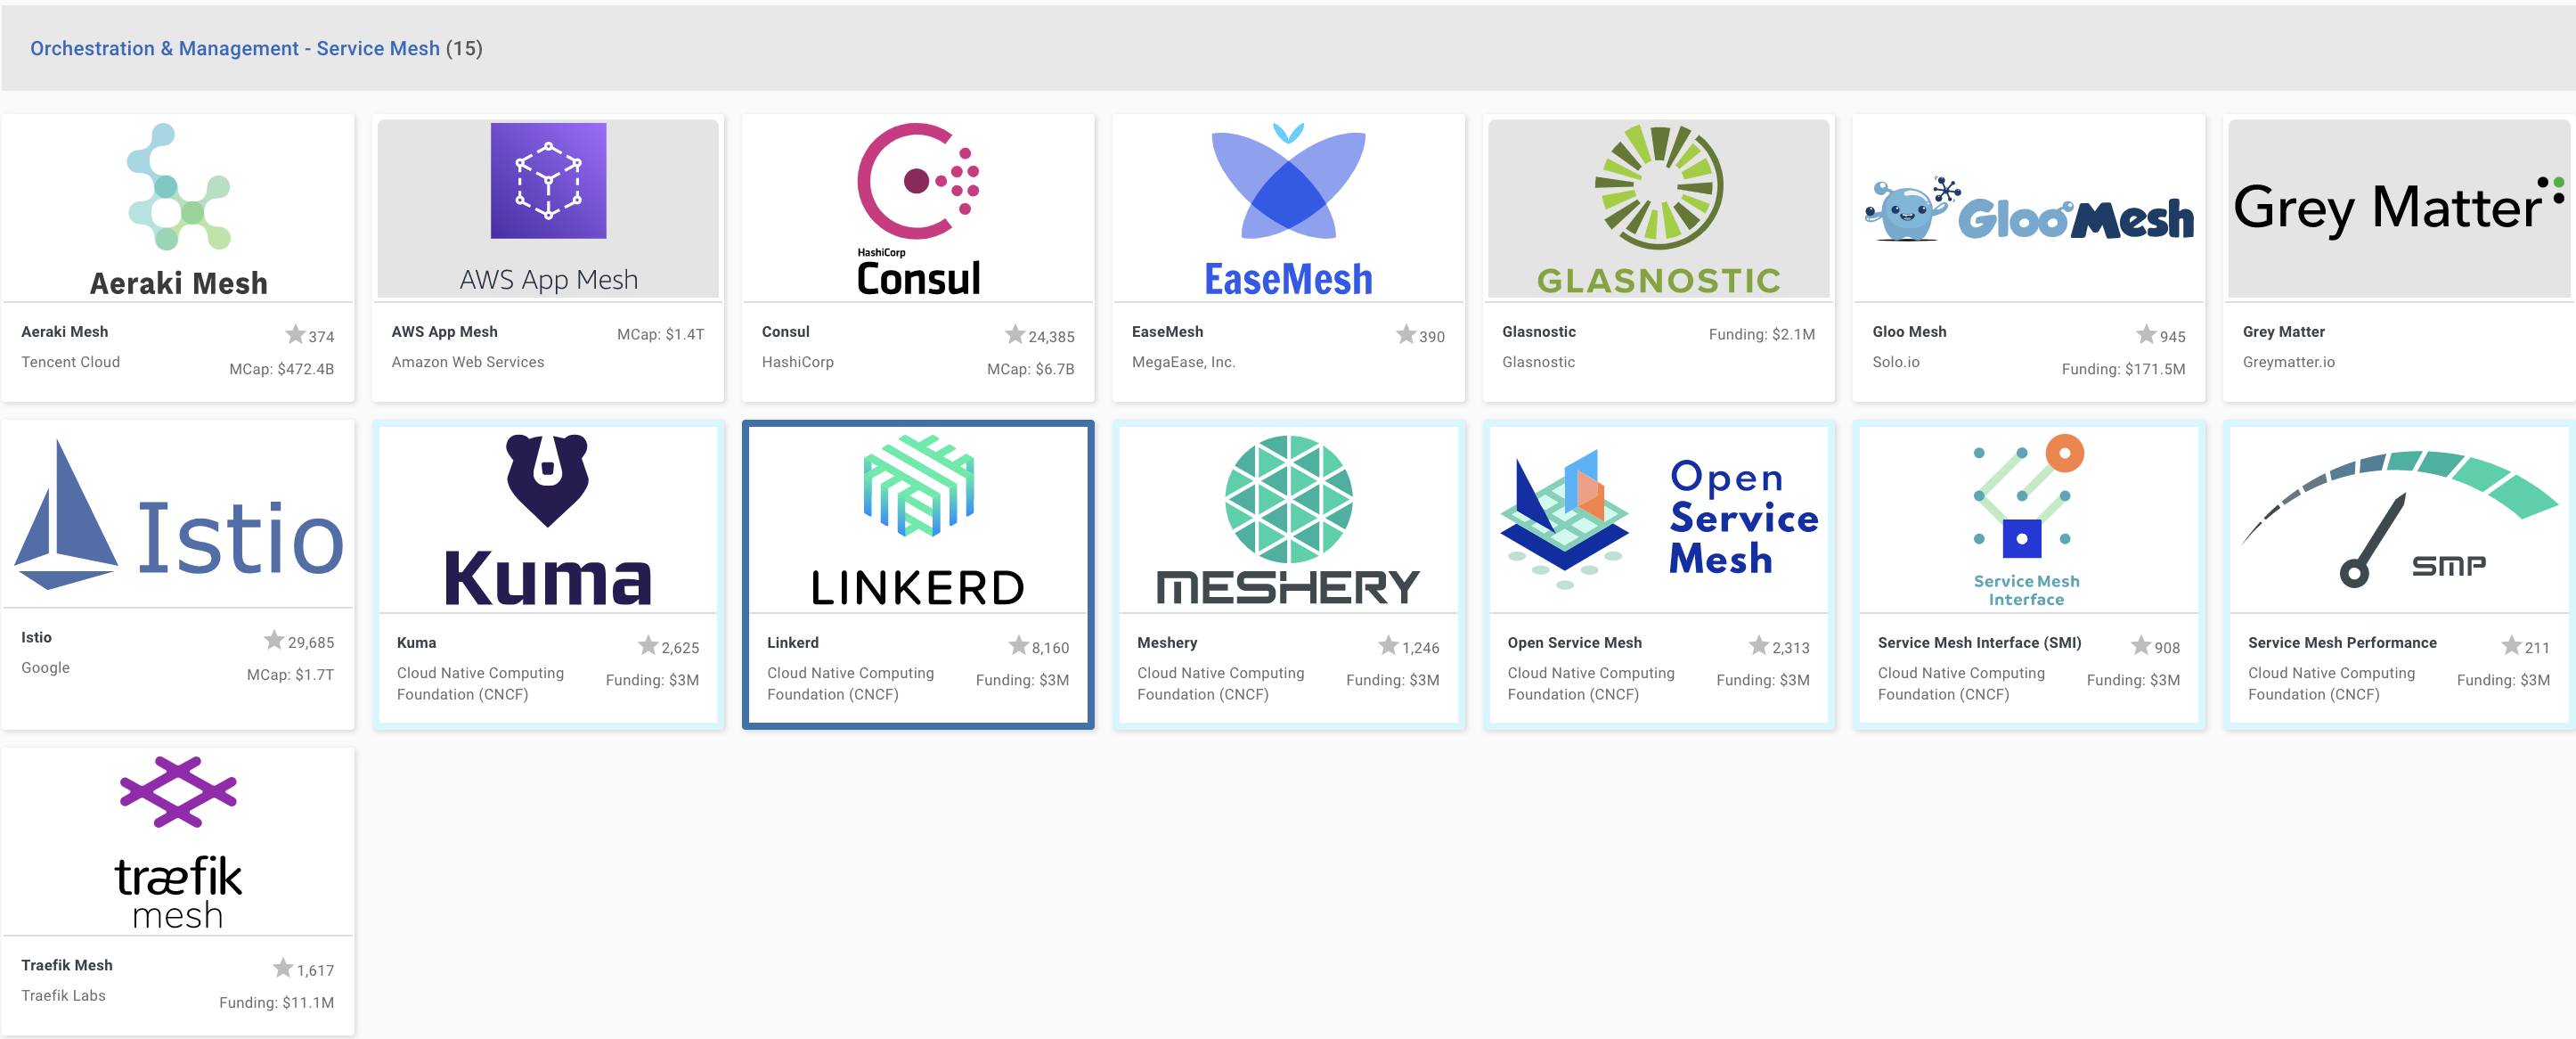
\includegraphics[width=0.9\linewidth]{3_systems_survey/figures/cncf-landscape-service-mesh}
    \caption{\gls{cncf} landscape of \gls{sm} technologies as of March 2022}
    \label{fig:cncf-landscape-sm}
\end{figure*}

% Conclude that there is a need for the review
% - Lack of formal (reiterate)
% - Industry interest
% - New approaches (proxyless, ebpf)
In order to justify a formal systematic survey, we have to evaluate the environment and related work. First, we have evaluated the existing formal literature in the field, as stated above, and concluded that this was lacking and unfit for the goals and research that we have in mind. Secondly, we evaluated the interest from within the community regarding the \gls{sm} technology. Our preliminary analysis showed that this was a sharp contrast against the interest from within the academic world. The field has an abundance of blog posts, talks, and the author of \gls{linkerd}, a popular \gls{sm} implementation, even went as far to call it “the world’s most over-hyped technology” \cite{service-mesh-hype}. Additionally, we found that the technology has received widespread adoption and interest from the industry, with a steady increase in production usage as indicated in surveys conducted by Red Hat \cite{rh-survey} and the \gls{cncf} \cite{cncf-survey-2020}. Finally, the very recent developments \cite{istio-merbridge, cilium-ebpf-mesh} in the field (less than two months old at the time of writing), which fundamentally change the approach, provide  interesting takes to survey this field at this very moment. This all results in a justification for conducting the survey, and that the timing of it manages to capture an interesting shift within the field.


\subsection{Goals}
\label{sec:survey:goals}
% What are we trying to achieve in this survey
% - Bridge the gap between academia and industry
% - Gain insights into the current state-of-the-art-systems
% - Obtain knowledge about relative metrics and workloads 
% - ^> Is a stepping stone to the next chapter

% - Tie it all to the research question defined in the introduction

Prior to conducting a systematic systems survey, we first establish a set of goals which we will try to achieve in this work. This allows us to structure the research and adjust its methodologies based on the goals. The following list represents the formulated goals.

\begin{enumerate}[label=\textbf{G\arabic*}, leftmargin=3\parindent]
    \item \textbf{Bridge the gap between academia and industry.}
    \label{g-1}
    
    In the previous section (\cref{sec:survey:related-work}), we identified that there is a large gap between interest from academia and the industry. We identified that there is a lack of formal publications in the field, whereas preliminary exploration showed that this is in sharp contrast to the interest as expressed from the industry. This leads to this first goal, which is to close this gap and provide formal research in this emerging field.
    
    \item \textbf{Gain insight into the current state-of-the-art \gls{sm} systems.}
    \label{g-2}
    
    The second goal of this survey is to gain a clear understanding of the field and the current state-of-the-art \gls{sm} systems. We want to identify the systems that currently exist and identify their defining properties and characteristics.

    \item \textbf{Obtain knowledge about relevant performance metrics.}
    \label{g-3}
    
    Finally, we want to identify metrics that properly capture the performance implications of these systems. By examining these systems in detail, we want to obtain the metrics which are relevant in the application domain. 

\end{enumerate}

% - Tie it all to the research question defined in the introduction
% - Tie it to the general flow of the thesis as this provides a stepping stone to further chapters
The goals and their respective order in which they are  presented are closely tied to the general flow of research conducted within this thesis. We first established the gap between industry and academia in our previous work \todo{cite prev work} and formulated this thesis around the idea to close this \ref{g-1}. Furthermore, we apply research best practices by conducting a survey of the field. This helps us to understand the field and allows us to examine the current state-of-the-art systems in detail \ref{g-2}. The data synthesis of this survey allows us to establish a framework to compare the existing and future \gls{sm} systems which might emerge. The results of this will be used to provide the answer to the research question \ref{rq-1} during our analysis. Additionally, the survey and resulting framework allows us to determine relevant metrics \ref{g-3}. This provides a stepping stone towards the following chapter, in which we design an instrument to compare the performance characteristics of these systems. \todo{cite next chapter if systems survey done}
\section{Methodology}
\label{sec:survey:methodology}

% General intro of what is happening in this chapter
% - Systematic approach to a survey (reproducible)
% - Section structure
The following section covers the methodology that is used throughout the systematic systems review. The idea of the systematic approach is to make the results as presented in this chapter reproducible. This is done by extensively detailing the methodology used and explaining the decisions we had to take. We present the guidelines, data sources and steps taken in order to reach the dataset used in the data synthesis. 

The remainder of this section is structured as follows. First, in \cref{sec:survey:methodology:strategy} we identify and discuss methods and techniques commonly used in systems surveys. Secondly, in \cref{sec:survey:methodology:approach}, we combine the methods and techniques identified, and present the strategy that we used to approach this survey. After that, we introduce the research protocol that we established to conduct the survey.




\subsection{Defining a Strategy}
\label{sec:survey:methodology:strategy}

% Introduction to strategy definition


There are many methods and techniques out there to find, select or synthesize the data for a survey. The methodology and technique used throughout such a survey ultimately dictates the form a survey takes on and influences the results it produces. It is important to identify, compare and choose such methods and techniques that fit the needs of our system-focussed survey. 

In this section, we will present the identified methods that we can use for a survey. For each method, we discuss their advantages and disadvantages and whether we will use them in some form within the survey.

\subsubsection{Unguided Techniques}
\label{sec:survey:methodology:strategy:unguided}

% Analysis of common survey methods
% - Unguided Methods
% - Unguided Search -> Initial dataset
% - Backward Snowballing -> Enhange datase


\textit{Unguided search} is the first technique that we have identified. This technique is commonly used to produce an initial dataset of relevant literature on the topic. This process requires the researcher to traverse various digital libraries equipped with relevant keywords to produce the dataset. Another commonly used technique that we have identified is \textit{backward snowballing}. This is another unguided method often used as a complementary technique in order to expand the dataset and is achieved by searching for related papers in the reference section. By combining these techniques, a researcher can create a literature review based on the generated dataset. However, both of the techniques are unguided, and therefore the process is not reproducible. Using such unguided techniques can result in completely different datasets if the process is to be repeated by another researcher, and thus does not produce much scientific value. 

% Analysis of common survey methods
% - Guided Methods
% - SLR (Kitchenham) -> Planning, Conducting, Reporting
% - Petersen -> comparative analysis guidelines
\subsubsection{Systematic Approach}
\label{sec:survey:methodology:strategy:systematic}

% SLR
In order to prevent any form of bias to have an effect on the process and results of a survey, we have to establish and utilize a systematic approach. We have identified a state-of-the-art methodology which aims to create a systematic process which will be used to guide this survey. The works of Kitchenham and Charters \cite{Kitchenham2007} introduce a battle-tested and auditable set of guidelines for literature reviews aimed at software engineering researchers  with the goal of promoting reproducibility. The introduced \gls{slr} methodology consists of three steps, planning the review, conducting the review and reporting the review. We decided to use these guidelines as a baseline for the survey, as it aligns with our goals and environment.

In addition to the guidelines introduced by the \gls{slr} methodology, we utilize the guidelines as introduced in the works of Petersen et al. \cite{Petersen2008}\cite{Petersen2015}. The authors introduce a set of guidelines and techniques which can be used to conduct a mapping study on a given topic. Among the guidelines and techniques, the authors introduce a method to perform comparative analysis. These guidelines and methods align with our needs and goals to compare \gls{sm} systems in the field as stated by the formulated research question \ref{rq-1}. 

% MLR method (Garousi)
% - MLR (Garousi) -> Inclusion of GL
\subsubsection{Inclusion of Grey Literature}
\label{sec:survey:methodology:strategy:gl}

% - Previous lit survey -> Lack of PL
% - 2019 Secondary survey -> Lack of PL
% - Most content from the industry is GL
One of the drawbacks of the \gls{slr} method is that it only concerns \gls{pl}, which consists of published peer-reviewed academic articles. In our previous work, in which we have conducted a systematic literature review on the \gls{k8s} ecosystem, we came to the conclusion that this field lacked published and peer-reviewed articles. Additionally, previous secondary studies on the field came to the same conclusion \cite{service-mesh-survey}. The lack of published (formal) literature in the field makes it impossible for us to conduct the research to an extent which satisfies our goals. This led us to explore additional forms of literature. \Gls{gl} is a form of literature that does not belong in the formal category, and can be in the form of blog posts, videos or white papers. Exploratory research has shown that inclusion of \gls{gl} can be beneficial to our research, as most of the literature is presented in such form by the industry.

% - Introduction to MLR
In order to maintain a systematic approach with the inclusion of \gls{gl}, we had to define or find additional guidelines that supported this requirement. We have identified the state-of-the-art method for conducting a survey which enabled the inclusion of \gls{gl}. The \gls{mlr} methodology as introduced by Garousi et al. \cite{Garousi2019} adapts and extends the \gls{slr} method from Kitchenham et al. so that it can include both forms of literature. 

% MLR checklist table
\begin{table*}[t]
\centering
\resizebox{\linewidth}{!}{ %< auto-adjusts font size to fill line
    \begin{tabular}{@{}lll@{}}
    \toprule
    \# & Question & Answer \\
    \midrule
    1 & Is the subject “complex” and not solvable by considering only the formal literature? & Yes \\
    2 & Is there a lack of volume or quality of evidence, or a lack of consensus of outcome measurement in the formal literature? & Yes \\
    3 & Is the contextual information important to the subject under study? & Yes \\
    4 & Is it the goal to validate or corroborate scientific outcomes with practical experiences? & Yes \\ 
    5 & Is it the goal to challenge assumptions or falsify results from practice using academic research or vice versa? & No \\ 
    6 & Would a synthesis of insights and evidence from the industrial and academic community be useful to one or even both communities? & Yes \\ 
    7 & Is there a large volume of practitioner sources indicating high practitioner interest in a topic? & Yes \\ 
    \bottomrule
    \end{tabular}
} %< \resizebox
\caption[Questionnaire to decide whether to include \gls{gl}. ]{Questionnaire from the works of Garoussi et al. \cite{Garousi2019}, which helps to decide whether to include \gls{gl} in a literature survey.}
\label{tab:mlr-checklist}
\end{table*}

% - MLR requriements checklist
Additionally, the authors have created a checklist which can be used to verify the need for inclusion of \gls{gl} within a survey. If one or more of the questions in the checklist is answered with a “yes”, it indicates that \gls{gl} can be beneficial to the survey. We answered the questions in the provided checklist and the results of this can be seen in \cref{tab:mlr-checklist}. These results reaffirmed our requirement for \gls{gl} throughout the survey and made us adapt the guidelines as described by the methodology.




\subsection{Our Approach to a Systematic Survey}
\label{sec:survey:methodology:approach}
%  Summarize entire approach and present figure that shows this
% - SLR Leeading
% - MLR -> inclusiong of GL
% - Petersen -> comparitive analysis

In the previous section (\cref{sec:survey:methodology:strategy}), we identified several methodologies and guidelines which we can use to conduct a survey. We explained why we have chosen some of these guidelines for our systems survey and how they could apply to our research goals. The resulting strategy can be seen in more detail in the form of a flow chart in  \cref{fig:survey-methodology}. This figure depicts two of the three stages in the \gls{slr} methodology, namely the planning phase and the conducting phase. It also lists all the deliverables of this systems survey (\designref{D1} - \designref{D5}). 

Up to this point, we have discussed two steps of the planning phase. This first step of the planning phase \designref{P1}, consists of establishing a need for the survey, which we did in \cref{sec:survey:related-work}. Next, we established our goals \ref{g-1} - \ref{g-3} and research question \ref{rq-1} in \cref{sec:survey:goals} which relates to process \designref{P2}.




% Support findings based on some perspectives
\begin{figure}[!t]
    \centering
    
    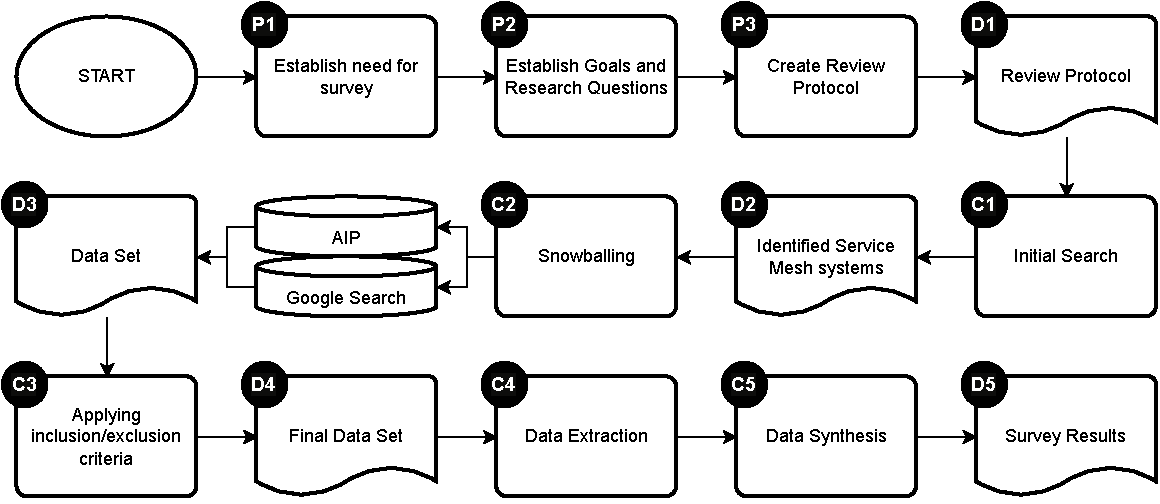
\includegraphics[width=\linewidth]{3_systems_survey/figures/survey-methodology}

    \caption{System Survey approach.}
    \label{fig:survey-methodology}
\end{figure}




% % SLR Plannign phase
% % 1. Investigate need (rel. work)
% % 2. Objective of this research
% % 3. Formulate RQ.
% \subsection{Planning}
% \label{sec:survey:methodology:planning}

% \todo{Fix planning section}

% In line with the guidelines as proposed in the \gls{slr} methodology, we first conducted a planning stage. During this stage we have analysed relevant work and the need for a review as discussed in \cref{sec:survey:related-work}. After this, we formulated the goal and related research question of this survey as seen in \cref{sec:survey:goals}. The goal of this systems survey is to uncover the existing \gls{sm} systems in the landscape and provide an overview of characteristics that they have. By creating a data synthesis of the literature that we are able to find on this topic, we can produce a general framework to contain these systems. This is a stepping stone for the research that is conducted in the later chapters, in which we examine and evaluate the characteristics and performance properties of these systems in more detail. 



% SLR - Review Protocol
\subsection{Review Protocol}
\label{sec:survey:methodology:review-protocol}

% Review protocol consists of
% - Background, the rationale for the survey -> Goals
% - Research Questions that we intend to answer


% PL & GL
% - Search Strategy
% - Selection Criteria
% - Selection Procedures
% - Data Extraction



The review protocol is a fundamental aspect of the \gls{slr} methodology, it specifies the methods used to conduct the systems review in this thesis. A pre-defined protocol is required to reduce the possibility of any bias. Establishing the review protocol is part of our approach as specified in \cref{fig:survey-methodology} and depicts the process \designref{P3}.

In the remainder of this section, we introduce the components that establish the research protocol. In \cref{sec:survey:methodology:review-protocol:search-strategy}, we introduce the search strategy which is used to search for the relevant literature. In \cref{sec:survey:methodology:review-protocol:selection-criteria}, we establish the selection criteria which are used to filter the dataset which we obtained through the research strategy. Finally, in \cref{sec:survey:methodology:review-protocol:data-extraction}, we describe the methods used to extract and synthesize the data.



\subsubsection{Search Strategy}
\label{sec:survey:methodology:review-protocol:search-strategy}
% - Data Sources
% - Queries

In order to create a reproducible data set, we have to establish a search strategy which we use to obtain literature on the topic. The search strategy differs based on the type of literature, where different requirements apply for \gls{pl} and \gls{gl}.


% Data sources
% - AIP
% - Digital Libraries (DBLP, Aminer, Semantic Scholar)
% - Only established, well respected conferences
The first component that makes up the search strategy is related to the data sources. The Atlarge  team\footnote{\url{https://atlarge-research.com/}} has identified several digital libraries which are well established and which contain the leading publications in the field of distributed systems. Additionally, years of experience in the field led to the creation of a list of established and well-respected conferences. This consolidated knowledge led to the development of a software instrument \gls{aip}. This instrument is used to generate the initial dataset of \gls{pl} for this survey and query it. To establish a dataset of \gls{gl} in this survey, we use Google Search to identify relevant literature.

The second component of the search strategy is related to the search technique. Since the goal of this survey to compare state-of-the-art \gls{sm} systems, we first have to identify said systems. In order to do that, we first conducted exploratory research in the field. In order to reduce bias in this process, we first used the single identified secondary study \cite{service-mesh-survey} to obtain an initial set of \gls{sm} systems. After this, we identified the \gls{sm} systems that were part of official \gls{cncf} projects\footnote{\url{https://landscape.cncf.io/card-mode?category=service-mesh&grouping=category}}, as they proved to be an authoritative entity in the field as discussed in \cref{sec:background:cncf}. This list was then complemented by results obtained from \gls{gl} using generic search queries. 


The final component of the search strategy is related to the search queries that we use to establish the resulting dataset. In order to find and identify the current state-of-the-art \gls{sm} systems, we used generic terms as described above. After this, we utilized a snowballing method in which we based the search queries on the identified systems. The final list of search queries used can be seen in \cref{tab:search-queries}. Queries \textbf{Q1} and \textbf{Q2} represent the queries used to obtain and expand the list of identified \gls{sm} systems, while \textbf{Q3} indicates the system specific queries that were used. 

\begin{table}[t]
\centering
% \resizebox{\linewidth}{!}{ %< auto-adjusts font size to fill line
    \begin{tabularx}{\linewidth}{lXl}
    \toprule
    \# & Query & Search Strategy \\
    
    % Initial Search Queries
    \midrule
    \textbf{Q1} & Service Mesh & Initial Search \\
    \textbf{Q2} & Service Mesh Implementation & Initial Search \\

    % Queries Based on identified SM systems
    \midrule
    \textbf{Q3} & \textit{Identified Service Mesh Implementation} & Snowballing  \\
    
    \bottomrule
    \end{tabularx}
% } %< \resizebox
\caption{Search queries established in the review protocol.}
\label{tab:search-queries}
\end{table}

% \begin{table}[t]
% \centering
% % \resizebox{\linewidth}{!}{ %< auto-adjusts font size to fill line
%     \begin{tabular}{@{}lll@{}}
%     \toprule
%     \# & Query & Search Strategy \\
    
%     % Initial Search Queries
%     \midrule
%     \textbf{Q1} & Service Mesh & Initial Search \\
%     \textbf{Q2} & Service Mesh Implementation & Initial Search \\

%     % Queries Based on identified SM systems
%     \midrule
%     \textbf{Q3} & \textit{Identified Service Mesh Implementation} & Snowballing  \\
    
%     \bottomrule
%     \end{tabular}
% % } %< \resizebox
% \caption{Search queries established in the review protocol.}
% \label{tab:search-queries}
% \end{table}



\subsubsection{Selection Criteria}
\label{sec:survey:methodology:review-protocol:selection-criteria}
% Seperate Criteria for PL and GL
% Introduce the checklist and how it works
% display PL and GL checklist
Since we have decided to also include \gls{gl} in our survey, we decided to establish two sets of selection criteria since they are vastly different in terms of content and medium. For both types of literature, we establish a checklist. In this checklist, we define the guidelines that we use to either include or exclude a data point. Guidelines prefixed with a checkmark (\cmark) symbol indicate a reason to include a publication in the research, whereas the cross (\xmark) symbol indicates a reason for exclusion. 

The following checklist (\cref{list:checklist:pl}) contains a set of selection criteria that applies to the \gls{pl} that is obtained through the search process. For this, we apply a set of generic criteria in order to 

In addition to the search queries, we used a filter to filter out any results before 2014 since that the initial release date of \gls{k8s} \cite{kubernetes-overview}. This limits the results based on the scope of this research, which provides a focus on \gls{sm} systems in a \gls{k8s} environment.

\begin{itemize}
    \item[(\cmark)] Publications that are written in English.
    \item[(\cmark)] Publications introducing novel concepts.
    \item[(\cmark)] Publications that focus on architectural problems and solutions.
    \item[(\cmark)] Publications performing performance analysis studies.
    
    \item[(\xmark)] Publications before 2014. 
    \item[(\xmark)] Publications that do not have \gls{sm} systems as the primary subject in the research. 
    \item[(\xmark)] Secondary or tertiary studies regarding \gls{sm} systems.
    \item[(\xmark)] Publications that are not full-text (e.g., small snippets or as part of a demo).
    
    \label{list:checklist:pl}
\end{itemize}


The following checklist (\cref{list:checklist:gl}) contains a set of selection criteria that applies to the \gls{gl} that is obtained through the search process. For this form of literature we had to establish a set of rigorous guidelines since it can otherwise result in numerous data entries or lead to a biased set of results. 

\begin{itemize}
    \item[(\cmark)] Publications that are written in English.
    \item[(\cmark)] Publications introducing novel concepts.
    \item[(\cmark)] Publications originating from well established and known organizations (e.g. \gls{cncf}, Google, Red Hat, etc.)
    \item[(\cmark)] Publications that supply official vendor or platform documentation
    \item[(\cmark)] Publications in the form of blog posts from organizations or authorities in the field.
    \item[(\cmark)] Publications in the form of videos from talks or conferences related to the field.
    \item[(\cmark)] Source code repositories of open-source \gls{sm} systems (e.g. a GitHub repository).
    
    \item[(\xmark)] Publications in which we cannot validate the authority of an author (e.g. anonymous posts, or posts by someone not established in the field). 
    \item[(\xmark)] Publications which do not provide any novelty for the survey (e.g. tutorials on the technologies). 
    \item[(\xmark)] Publications that are not full-text (e.g., small snippets, parts of a demo or short social media excerpts such as tweets).
    
    \label{list:checklist:gl}
\end{itemize}


\subsubsection{Data Extraction}
\label{sec:survey:methodology:review-protocol:data-extraction}
% What kind of information is relevant to us
% Compare systems
% Observability
% Resilience
% Proxy Characteristics
% Protocol Support
% Security
% Meta


Once we have established a final dataset by filtering the dataset based on the selection criteria, we can start the data synthesis process. To achieve this, we first have to establish a set of data extraction guidelines. These guidelines have to be in line with the goals which of this survey. Since we want to compare existing state-of-the-art \gls{sm} systems, we have to identify the key characteristics and properties  of such systems. Through the preliminary research conducted on the field, we understand the fundamentals of a \gls{sm} system and have identified the challenges it tries to solve. With this in mind, we try to identify and synthesize the data based on key areas.


% Observability
% Resilience
% Proxy Characteristics
% Protocol Support
% Security
% Meta
First off, we try to compare these systems based on their architectural approach. With this take, we can identify and compare \gls{sm} systems based on their design decisions, such as their control and data plane components. Secondly, we take a functional approach to synthesize these systems. By identifying sets of functionality, we can evaluate and compare these systems on domain-specific functionalities such as their observability, security or resiliency characteristics. Furthermore, we take a meta analytical approach to these systems. With this, we try to establish certain aspects such as the number of users the system has, the development activity on the project, whether a project is open-source or not and the maturity of the system.
\section{Results}
\label{sec:survey:results}
\section{Analysis of state-of-the-art \gls{sm} systems.}
\label{sec:survey:analysis}